\documentclass{article}
\usepackage{ctex}
\usepackage{geometry}
\geometry{a4paper, scale=0.8}
\usepackage{graphicx}
\usepackage{subfigure}
\usepackage{float}
\usepackage{enumitem}
\usepackage{amsmath}
\usepackage{amssymb}

\title{HW02}
\author{PB19071405\ 王昊元}
\date{2022 年 04 月 28 日}

\begin{document}
    \maketitle

    \begin{enumerate}[label=\arabic*.]
        \item 类图如下:\\
        \begin{figure}[H]
            \centering
            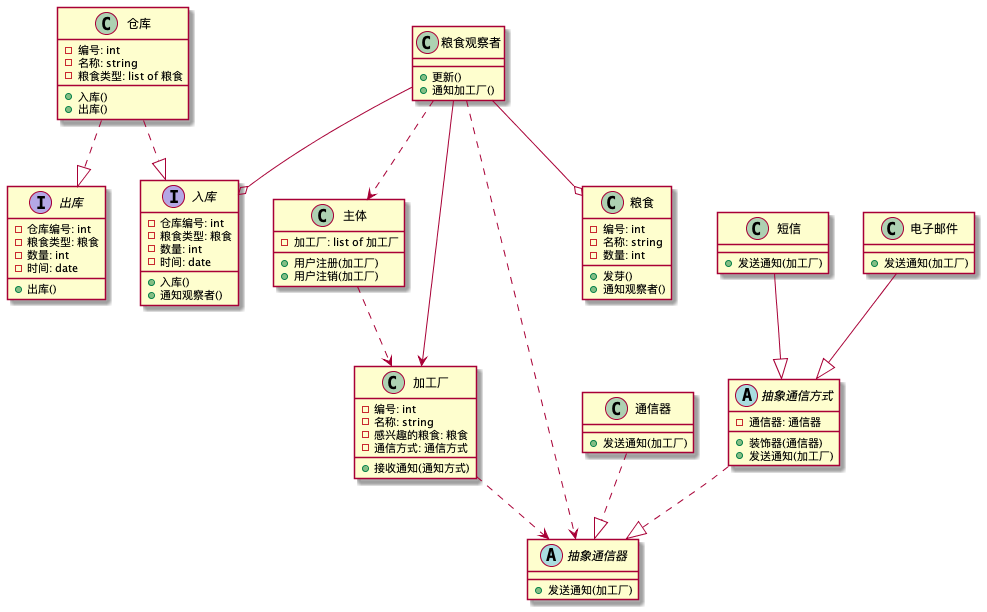
\includegraphics[width=0.7\textwidth]{./fig/hw02/1.png}
            \caption{智能仓储GES系统类图}
        \end{figure}
        类图说明如下:(有画的或设计的不合适的地方,还烦请助教指出)\\
        \begin{itemize}
            \item 仓库:表示仓库的类,记录仓库自身及内部粮食信息,可进行入库出库操作
            \item 入库、出库:入库出库操作的接口
            \item 主体:表示主体模块的类,记录加工厂登记的信息,可进行用户注册和注销操作
            \item 加工厂:表示加工厂的类,记录加工厂具体信息(可实例化为一个个具体的加工厂),可接收通信器发的通知
            \item 粮食:表示粮食的类,记录粮食具体信息,会发芽(进行发芽操作)
            \item 粮食观察者:观察者模式中的observer,观察粮食是否发芽及是否发生入库操作,在需要时通知加工厂
            \item 抽象通信器:通信器的抽象类,装饰器模式中的抽象组件
            \item 通信器:代表通信器的类,装饰器模式中的具体组件
            \item 抽象通信方式:通信方式的抽象类,装饰器模式中的抽象装饰
            \item 短信、电子邮件:代表各种具体通信方式的类,装饰器模式中的具体装饰,
            在通信方式有变化时可以新建一种类代表新的通信方式,通过装饰器模式可以方便地更新通信方式
        \end{itemize}
        \item 类图如下:\\
        \begin{figure}[H]
            \centering
            % 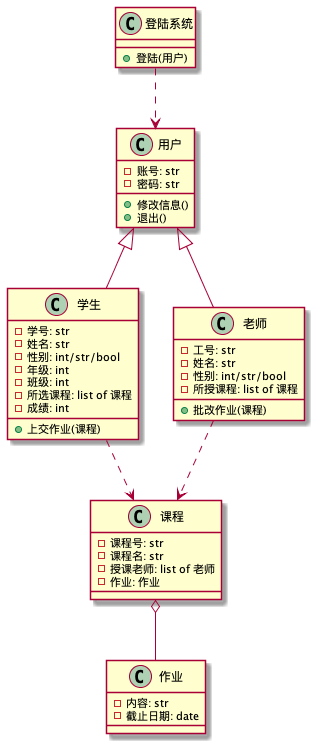
\includegraphics[width=0.7\textwidth]{./fig/hw02/2.png}
            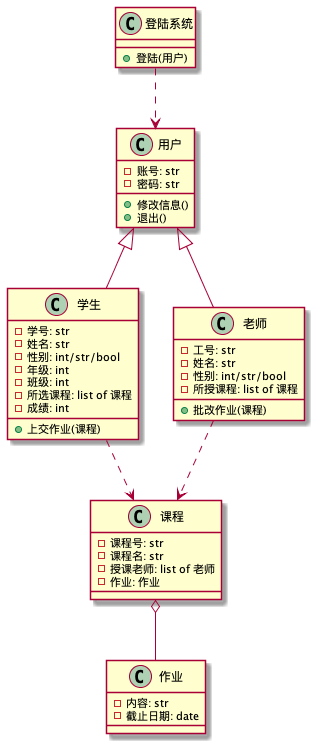
\includegraphics[scale=0.5]{./fig/hw02/2.png}
            \caption{线上教育系统类图}
        \end{figure}
        类图说明如下:\\
        \begin{itemize}
            \item 登陆系统:登陆系统地类,可进行登陆操作
            \item 用户:代表者用户的类,可进行修改信息和退出的类
            \item 学生:一类特殊的用户,代表学生的类,可进行上交作业的操作
            \item 老师:一类特殊的用户,代表老师的类,可进行批改作业的操作
            \item 课程:代表课程的类,包含了课程具体信息
            \item 作业:代表作业的类,包含了作业的具体信息
        \end{itemize}
        学生提交作业的时序图如下:\\
        \begin{figure}[H]
            \centering
            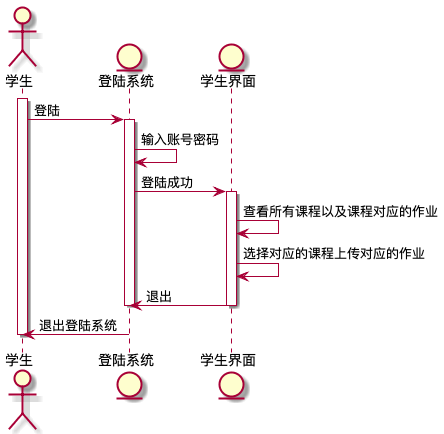
\includegraphics[width=0.7\textwidth]{./fig/hw02/2_student.png}
            \caption{学生提交作业时序图}
        \end{figure}
        老师批改作业的时序图如下:\\
        \begin{figure}[H]
            \centering
            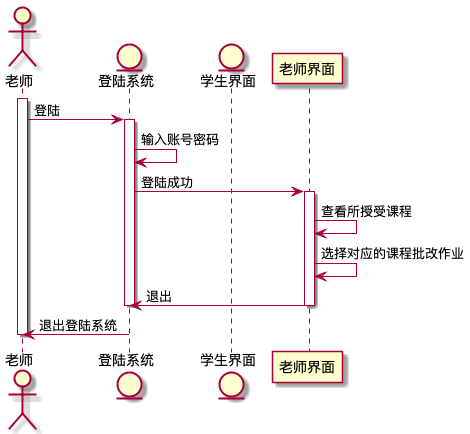
\includegraphics[width=0.7\textwidth]{./fig/hw02/2_teacher.png}
            \caption{老师批改作业时序图}
        \end{figure}
    \end{enumerate}
\end{document}
